\documentclass[twoside]{book}

% Packages required by doxygen
\usepackage{fixltx2e}
\usepackage{calc}
\usepackage{doxygen}
\usepackage[export]{adjustbox} % also loads graphicx
\usepackage{graphicx}
\usepackage[utf8]{inputenc}
\usepackage{makeidx}
\usepackage{multicol}
\usepackage{multirow}
\PassOptionsToPackage{warn}{textcomp}
\usepackage{textcomp}
\usepackage[nointegrals]{wasysym}
\usepackage[table]{xcolor}

% Font selection
\usepackage[T1]{fontenc}
\usepackage[scaled=.90]{helvet}
\usepackage{courier}
\usepackage{amssymb}
\usepackage{sectsty}
\renewcommand{\familydefault}{\sfdefault}
\allsectionsfont{%
  \fontseries{bc}\selectfont%
  \color{darkgray}%
}
\renewcommand{\DoxyLabelFont}{%
  \fontseries{bc}\selectfont%
  \color{darkgray}%
}
\newcommand{\+}{\discretionary{\mbox{\scriptsize$\hookleftarrow$}}{}{}}

% Page & text layout
\usepackage{geometry}
\geometry{%
  a4paper,%
  top=2.5cm,%
  bottom=2.5cm,%
  left=2.5cm,%
  right=2.5cm%
}
\tolerance=750
\hfuzz=15pt
\hbadness=750
\setlength{\emergencystretch}{15pt}
\setlength{\parindent}{0cm}
\setlength{\parskip}{0.2cm}
\makeatletter
\renewcommand{\paragraph}{%
  \@startsection{paragraph}{4}{0ex}{-1.0ex}{1.0ex}{%
    \normalfont\normalsize\bfseries\SS@parafont%
  }%
}
\renewcommand{\subparagraph}{%
  \@startsection{subparagraph}{5}{0ex}{-1.0ex}{1.0ex}{%
    \normalfont\normalsize\bfseries\SS@subparafont%
  }%
}
\makeatother

% Headers & footers
\usepackage{fancyhdr}
\pagestyle{fancyplain}
\fancyhead[LE]{\fancyplain{}{\bfseries\thepage}}
\fancyhead[CE]{\fancyplain{}{}}
\fancyhead[RE]{\fancyplain{}{\bfseries\leftmark}}
\fancyhead[LO]{\fancyplain{}{\bfseries\rightmark}}
\fancyhead[CO]{\fancyplain{}{}}
\fancyhead[RO]{\fancyplain{}{\bfseries\thepage}}
\fancyfoot[LE]{\fancyplain{}{}}
\fancyfoot[CE]{\fancyplain{}{}}
\fancyfoot[RE]{\fancyplain{}{\bfseries\scriptsize Generated by Doxygen }}
\fancyfoot[LO]{\fancyplain{}{\bfseries\scriptsize Generated by Doxygen }}
\fancyfoot[CO]{\fancyplain{}{}}
\fancyfoot[RO]{\fancyplain{}{}}
\renewcommand{\footrulewidth}{0.4pt}
\renewcommand{\chaptermark}[1]{%
  \markboth{#1}{}%
}
\renewcommand{\sectionmark}[1]{%
  \markright{\thesection\ #1}%
}

% Indices & bibliography
\usepackage{natbib}
\usepackage[titles]{tocloft}
\setcounter{tocdepth}{3}
\setcounter{secnumdepth}{5}
\makeindex

% Hyperlinks (required, but should be loaded last)
\usepackage{ifpdf}
\ifpdf
  \usepackage[pdftex,pagebackref=true]{hyperref}
\else
  \usepackage[ps2pdf,pagebackref=true]{hyperref}
\fi
\hypersetup{%
  colorlinks=true,%
  linkcolor=blue,%
  citecolor=blue,%
  unicode%
}

% Custom commands
\newcommand{\clearemptydoublepage}{%
  \newpage{\pagestyle{empty}\cleardoublepage}%
}

\usepackage{caption}
\captionsetup{labelsep=space,justification=centering,font={bf},singlelinecheck=off,skip=4pt,position=top}

%===== C O N T E N T S =====

\begin{document}

% Titlepage & ToC
\hypersetup{pageanchor=false,
             bookmarks=true,
             bookmarksnumbered=true,
             pdfencoding=unicode
            }
\pagenumbering{roman}
\begin{titlepage}
\vspace*{7cm}
\begin{center}%
{\Large My Project }\\
\vspace*{1cm}
{\large Generated by Doxygen 1.8.11}\\
\end{center}
\end{titlepage}
\clearemptydoublepage
\tableofcontents
\clearemptydoublepage
\pagenumbering{arabic}
\hypersetup{pageanchor=true}

%--- Begin generated contents ---
\chapter{Hierarchical Index}
\section{Class Hierarchy}
This inheritance list is sorted roughly, but not completely, alphabetically\+:\begin{DoxyCompactList}
\item \contentsline{section}{Character\+Prototype}{\pageref{classCharacterPrototype}}{}
\begin{DoxyCompactList}
\item \contentsline{section}{A\+I\+Character}{\pageref{classAICharacter}}{}
\item \contentsline{section}{Playable\+Character}{\pageref{classPlayableCharacter}}{}
\end{DoxyCompactList}
\item \contentsline{section}{Character\+Prototype\+Factory}{\pageref{classCharacterPrototypeFactory}}{}
\item Message\begin{DoxyCompactList}
\item \contentsline{section}{Character}{\pageref{classCharacter}}{}
\item \contentsline{section}{Character\+List}{\pageref{classCharacterList}}{}
\end{DoxyCompactList}
\item \contentsline{section}{Static\+Descriptor\+Initializer\+\_\+\+Character\+Protobuf\+\_\+2eproto}{\pageref{structStaticDescriptorInitializer__CharacterProtobuf__2eproto}}{}
\end{DoxyCompactList}

\chapter{Class Index}
\section{Class List}
Here are the classes, structs, unions and interfaces with brief descriptions\+:\begin{DoxyCompactList}
\item\contentsline{section}{\hyperlink{classAICharacter}{A\+I\+Character} }{\pageref{classAICharacter}}{}
\item\contentsline{section}{\hyperlink{classCharacter}{Character} }{\pageref{classCharacter}}{}
\item\contentsline{section}{\hyperlink{classCharacterList}{Character\+List} }{\pageref{classCharacterList}}{}
\item\contentsline{section}{\hyperlink{classCharacterPrototype}{Character\+Prototype} }{\pageref{classCharacterPrototype}}{}
\item\contentsline{section}{\hyperlink{classCharacterPrototypeFactory}{Character\+Prototype\+Factory} }{\pageref{classCharacterPrototypeFactory}}{}
\item\contentsline{section}{\hyperlink{classPlayableCharacter}{Playable\+Character} }{\pageref{classPlayableCharacter}}{}
\item\contentsline{section}{\hyperlink{structStaticDescriptorInitializer__CharacterProtobuf__2eproto}{Static\+Descriptor\+Initializer\+\_\+\+Character\+Protobuf\+\_\+2eproto} }{\pageref{structStaticDescriptorInitializer__CharacterProtobuf__2eproto}}{}
\end{DoxyCompactList}

\chapter{Class Documentation}
\hypertarget{classAICharacter}{}\section{A\+I\+Character Class Reference}
\label{classAICharacter}\index{A\+I\+Character@{A\+I\+Character}}


{\ttfamily \#include $<$A\+I\+Character.\+h$>$}

Inheritance diagram for A\+I\+Character\+:\begin{figure}[H]
\begin{center}
\leavevmode
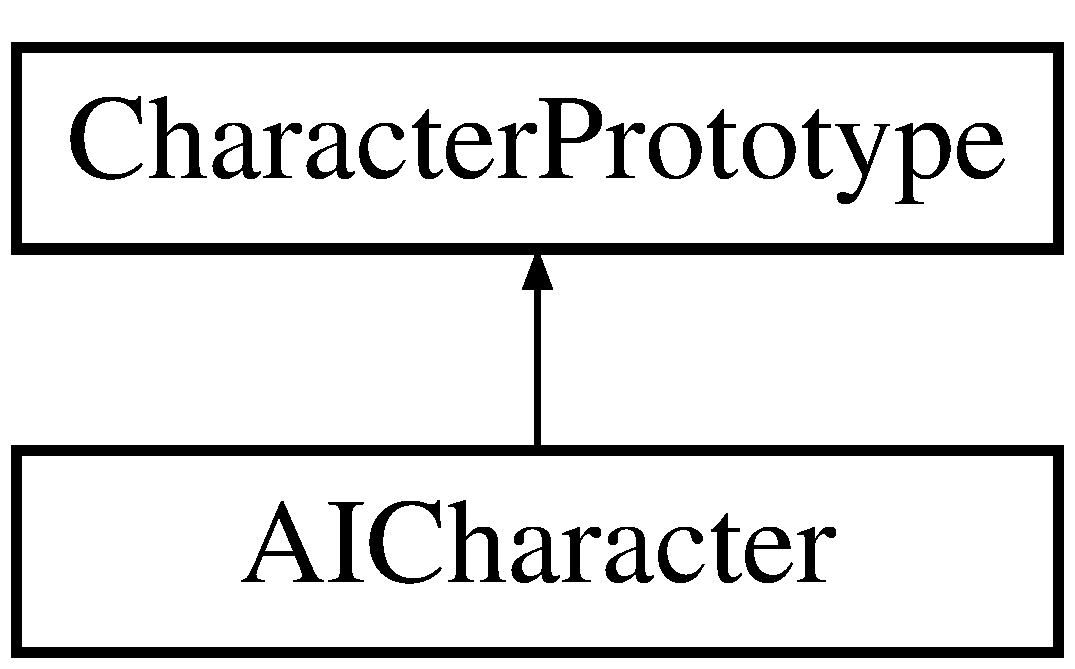
\includegraphics[height=2.000000cm]{classAICharacter}
\end{center}
\end{figure}
\subsection*{Public Member Functions}
\begin{DoxyCompactItemize}
\item 
\hyperlink{classAICharacter_a915c9436182d94bf6f6e1f3ffb11a319}{A\+I\+Character} (std\+::string name)
\item 
\hyperlink{classAICharacter_a20f8f8c486041489b7790ee25d57901e}{A\+I\+Character} (const \hyperlink{classAICharacter}{A\+I\+Character} \&orig)
\item 
virtual \hyperlink{classCharacterPrototype}{Character\+Prototype} $\ast$ \hyperlink{classAICharacter_a99b6f645c4e1f24d9701bac8f0dee596}{clone} ()
\item 
virtual \hyperlink{classAICharacter_ac270cee21ac69ed829cfc7b3c7f4c1b7}{$\sim$\+A\+I\+Character} ()
\end{DoxyCompactItemize}
\subsection*{Additional Inherited Members}


\subsection{Detailed Description}
An AI \hyperlink{classCharacter}{Character}, a derived class from the \hyperlink{classCharacterPrototype}{Character\+Prototype} 

\subsection{Constructor \& Destructor Documentation}
\index{A\+I\+Character@{A\+I\+Character}!A\+I\+Character@{A\+I\+Character}}
\index{A\+I\+Character@{A\+I\+Character}!A\+I\+Character@{A\+I\+Character}}
\subsubsection[{A\+I\+Character(std\+::string name)}]{\setlength{\rightskip}{0pt plus 5cm}A\+I\+Character\+::\+A\+I\+Character (
\begin{DoxyParamCaption}
\item[{std\+::string}]{name}
\end{DoxyParamCaption}
)}\hypertarget{classAICharacter_a915c9436182d94bf6f6e1f3ffb11a319}{}\label{classAICharacter_a915c9436182d94bf6f6e1f3ffb11a319}
Creates a new AI \hyperlink{classCharacter}{Character} 
\begin{DoxyParams}{Parameters}
{\em name} & the name of the player \\
\hline
\end{DoxyParams}
\index{A\+I\+Character@{A\+I\+Character}!A\+I\+Character@{A\+I\+Character}}
\index{A\+I\+Character@{A\+I\+Character}!A\+I\+Character@{A\+I\+Character}}
\subsubsection[{A\+I\+Character(const A\+I\+Character \&orig)}]{\setlength{\rightskip}{0pt plus 5cm}A\+I\+Character\+::\+A\+I\+Character (
\begin{DoxyParamCaption}
\item[{const {\bf A\+I\+Character} \&}]{orig}
\end{DoxyParamCaption}
)}\hypertarget{classAICharacter_a20f8f8c486041489b7790ee25d57901e}{}\label{classAICharacter_a20f8f8c486041489b7790ee25d57901e}
Copies the AI player 
\begin{DoxyParams}{Parameters}
{\em orig} & the AI to copy \\
\hline
\end{DoxyParams}
\index{A\+I\+Character@{A\+I\+Character}!````~A\+I\+Character@{$\sim$\+A\+I\+Character}}
\index{````~A\+I\+Character@{$\sim$\+A\+I\+Character}!A\+I\+Character@{A\+I\+Character}}
\subsubsection[{$\sim$\+A\+I\+Character()}]{\setlength{\rightskip}{0pt plus 5cm}A\+I\+Character\+::$\sim$\+A\+I\+Character (
\begin{DoxyParamCaption}
{}
\end{DoxyParamCaption}
)\hspace{0.3cm}{\ttfamily [virtual]}}\hypertarget{classAICharacter_ac270cee21ac69ed829cfc7b3c7f4c1b7}{}\label{classAICharacter_ac270cee21ac69ed829cfc7b3c7f4c1b7}
Destroys the AI 

\subsection{Member Function Documentation}
\index{A\+I\+Character@{A\+I\+Character}!clone@{clone}}
\index{clone@{clone}!A\+I\+Character@{A\+I\+Character}}
\subsubsection[{clone()}]{\setlength{\rightskip}{0pt plus 5cm}{\bf Character\+Prototype} $\ast$ A\+I\+Character\+::clone (
\begin{DoxyParamCaption}
{}
\end{DoxyParamCaption}
)\hspace{0.3cm}{\ttfamily [virtual]}}\hypertarget{classAICharacter_a99b6f645c4e1f24d9701bac8f0dee596}{}\label{classAICharacter_a99b6f645c4e1f24d9701bac8f0dee596}
Clones the AI returns the base class \begin{DoxyReturn}{Returns}
the clone 
\end{DoxyReturn}


Implements \hyperlink{classCharacterPrototype_a7c3db310af19ff8c80eb3a7f20bd9986}{Character\+Prototype}.



The documentation for this class was generated from the following files\+:\begin{DoxyCompactItemize}
\item 
A\+I\+Character.\+h\item 
A\+I\+Character.\+cpp\end{DoxyCompactItemize}

\hypertarget{classCharacter}{}\section{Character Class Reference}
\label{classCharacter}\index{Character@{Character}}
Inheritance diagram for Character\+:\begin{figure}[H]
\begin{center}
\leavevmode
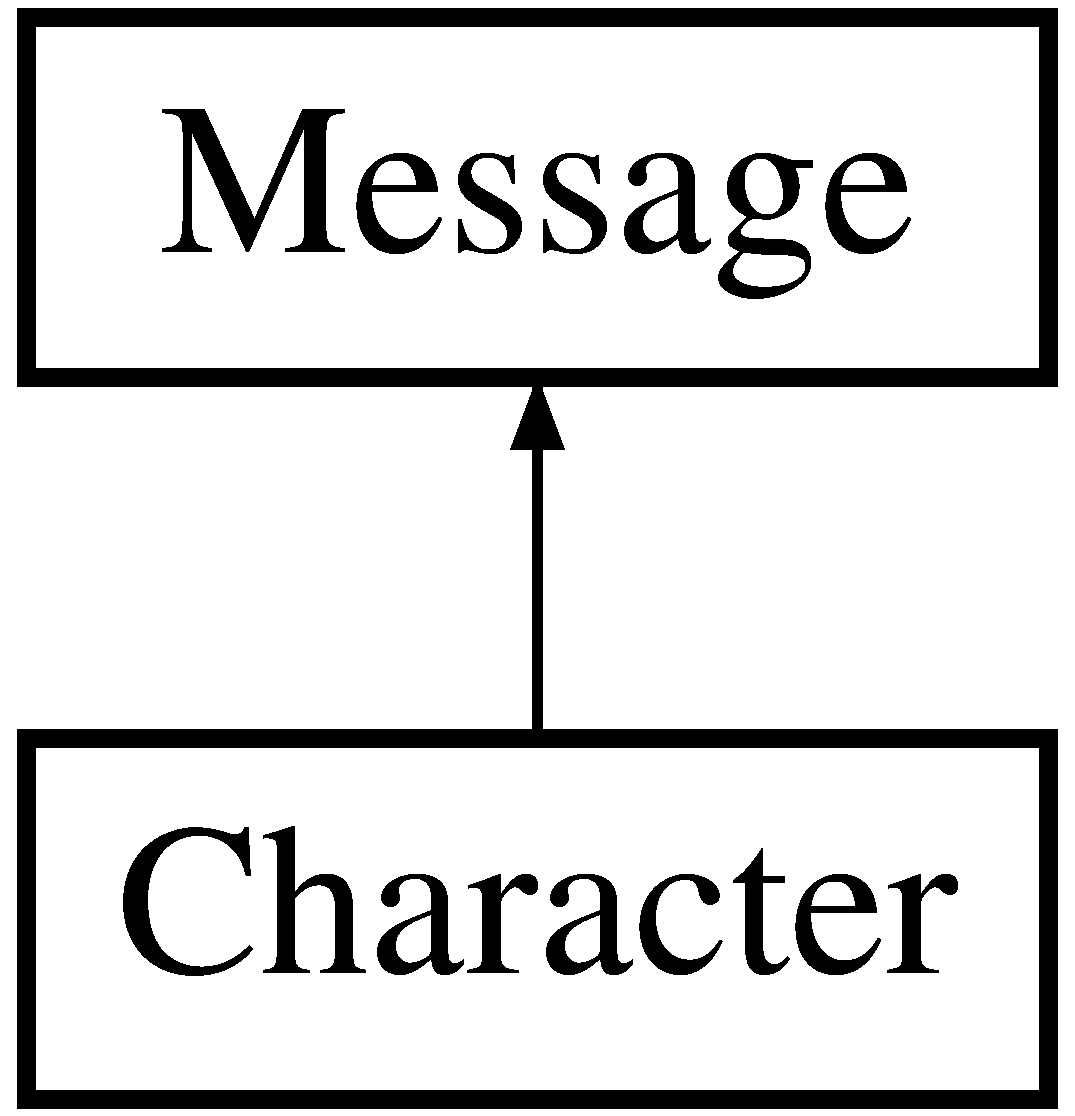
\includegraphics[height=2.000000cm]{classCharacter}
\end{center}
\end{figure}
\subsection*{Public Types}
\begin{DoxyCompactItemize}
\item 
typedef Character\+\_\+\+Type {\bfseries Type}\hypertarget{classCharacter_a1087098b8b7dfecf877b4fae559e4fd4}{}\label{classCharacter_a1087098b8b7dfecf877b4fae559e4fd4}

\end{DoxyCompactItemize}
\subsection*{Public Member Functions}
\begin{DoxyCompactItemize}
\item 
{\bfseries Character} (const \hyperlink{classCharacter}{Character} \&from)\hypertarget{classCharacter_a8f5bf8d77951e0ea45b39462a7546cdf}{}\label{classCharacter_a8f5bf8d77951e0ea45b39462a7546cdf}

\item 
\hyperlink{classCharacter}{Character} \& {\bfseries operator=} (const \hyperlink{classCharacter}{Character} \&from)\hypertarget{classCharacter_aab229e15048a97ef8ff087125ccaadcf}{}\label{classCharacter_aab229e15048a97ef8ff087125ccaadcf}

\item 
const \+::google\+::protobuf\+::\+Unknown\+Field\+Set \& {\bfseries unknown\+\_\+fields} () const \hypertarget{classCharacter_a579a66025abb75ec9020de5cf981b4cb}{}\label{classCharacter_a579a66025abb75ec9020de5cf981b4cb}

\item 
inline\+::google\+::protobuf\+::\+Unknown\+Field\+Set $\ast$ {\bfseries mutable\+\_\+unknown\+\_\+fields} ()\hypertarget{classCharacter_a9885e1f3fa422149a1fc6936616df9e1}{}\label{classCharacter_a9885e1f3fa422149a1fc6936616df9e1}

\item 
void {\bfseries Swap} (\hyperlink{classCharacter}{Character} $\ast$other)\hypertarget{classCharacter_ae439e522739760c54ef9d65acd53615e}{}\label{classCharacter_ae439e522739760c54ef9d65acd53615e}

\item 
\hyperlink{classCharacter}{Character} $\ast$ {\bfseries New} () const \hypertarget{classCharacter_af1c934cc12cbef7ddcf73bf7197cd3db}{}\label{classCharacter_af1c934cc12cbef7ddcf73bf7197cd3db}

\item 
void {\bfseries Copy\+From} (const \+::google\+::protobuf\+::\+Message \&from)\hypertarget{classCharacter_aa0496b0a8682360a40607c8f5b092875}{}\label{classCharacter_aa0496b0a8682360a40607c8f5b092875}

\item 
void {\bfseries Merge\+From} (const \+::google\+::protobuf\+::\+Message \&from)\hypertarget{classCharacter_a88ccb78cc0e4e17cb9287278cd4f6ed5}{}\label{classCharacter_a88ccb78cc0e4e17cb9287278cd4f6ed5}

\item 
void {\bfseries Copy\+From} (const \hyperlink{classCharacter}{Character} \&from)\hypertarget{classCharacter_add0afd0f841d005acea8326ca2028d90}{}\label{classCharacter_add0afd0f841d005acea8326ca2028d90}

\item 
void {\bfseries Merge\+From} (const \hyperlink{classCharacter}{Character} \&from)\hypertarget{classCharacter_adcf70ea964c51f2608063282baeaa607}{}\label{classCharacter_adcf70ea964c51f2608063282baeaa607}

\item 
void {\bfseries Clear} ()\hypertarget{classCharacter_a42a81f720f0dc1c2e5f0ac1c03ce3251}{}\label{classCharacter_a42a81f720f0dc1c2e5f0ac1c03ce3251}

\item 
bool {\bfseries Is\+Initialized} () const \hypertarget{classCharacter_a99242fb29ccace1bd0e21f3a79c954fb}{}\label{classCharacter_a99242fb29ccace1bd0e21f3a79c954fb}

\item 
int {\bfseries Byte\+Size} () const \hypertarget{classCharacter_af8c367cdffe969e07ad8917b5a107545}{}\label{classCharacter_af8c367cdffe969e07ad8917b5a107545}

\item 
bool {\bfseries Merge\+Partial\+From\+Coded\+Stream} (\+::google\+::protobuf\+::io\+::\+Coded\+Input\+Stream $\ast$input)\hypertarget{classCharacter_a9a96e8b83784508722e34b21172c7c57}{}\label{classCharacter_a9a96e8b83784508722e34b21172c7c57}

\item 
void {\bfseries Serialize\+With\+Cached\+Sizes} (\+::google\+::protobuf\+::io\+::\+Coded\+Output\+Stream $\ast$output) const \hypertarget{classCharacter_a922061bd15e72f5289a3d08f0fee7002}{}\label{classCharacter_a922061bd15e72f5289a3d08f0fee7002}

\item 
\+::google\+::protobuf\+::uint8 $\ast$ {\bfseries Serialize\+With\+Cached\+Sizes\+To\+Array} (\+::google\+::protobuf\+::uint8 $\ast$output) const \hypertarget{classCharacter_a0d5473252d5df1e2093474324c05f1e3}{}\label{classCharacter_a0d5473252d5df1e2093474324c05f1e3}

\item 
int {\bfseries Get\+Cached\+Size} () const \hypertarget{classCharacter_aed109b1efca920ee333712746bcfd256}{}\label{classCharacter_aed109b1efca920ee333712746bcfd256}

\item 
\+::google\+::protobuf\+::\+Metadata {\bfseries Get\+Metadata} () const \hypertarget{classCharacter_a131cbcdb689033b8696fce65d0b890c0}{}\label{classCharacter_a131cbcdb689033b8696fce65d0b890c0}

\item 
bool {\bfseries has\+\_\+name} () const \hypertarget{classCharacter_a81f2370d98998e7ad54c2df56fd2e7a1}{}\label{classCharacter_a81f2370d98998e7ad54c2df56fd2e7a1}

\item 
void {\bfseries clear\+\_\+name} ()\hypertarget{classCharacter_a0104106d7a1721d43d7e94b2e88b05a0}{}\label{classCharacter_a0104106d7a1721d43d7e94b2e88b05a0}

\item 
const \+::std\+::string \& {\bfseries name} () const \hypertarget{classCharacter_a2fb69b14ccc7b6a856f6d3a98d2b7261}{}\label{classCharacter_a2fb69b14ccc7b6a856f6d3a98d2b7261}

\item 
void {\bfseries set\+\_\+name} (const \+::std\+::string \&value)\hypertarget{classCharacter_a7d0f6be8e73483c4aac1e5a1a08b871d}{}\label{classCharacter_a7d0f6be8e73483c4aac1e5a1a08b871d}

\item 
void {\bfseries set\+\_\+name} (const char $\ast$value)\hypertarget{classCharacter_af1498f77a643ce021f654d744ef40bf6}{}\label{classCharacter_af1498f77a643ce021f654d744ef40bf6}

\item 
void {\bfseries set\+\_\+name} (const char $\ast$value, size\+\_\+t size)\hypertarget{classCharacter_acfedcef5579d06f0786b796e6c48fa1d}{}\label{classCharacter_acfedcef5579d06f0786b796e6c48fa1d}

\item 
inline\+::std\+::string $\ast$ {\bfseries mutable\+\_\+name} ()\hypertarget{classCharacter_ac829c93bde83f8f42cd1ba8d365caef3}{}\label{classCharacter_ac829c93bde83f8f42cd1ba8d365caef3}

\item 
inline\+::std\+::string $\ast$ {\bfseries release\+\_\+name} ()\hypertarget{classCharacter_a9d973d4b710de4c6ab00cb6b4c754083}{}\label{classCharacter_a9d973d4b710de4c6ab00cb6b4c754083}

\item 
void {\bfseries set\+\_\+allocated\+\_\+name} (\+::std\+::string $\ast$name)\hypertarget{classCharacter_a02ef1f00b4c9f65af29605911839db17}{}\label{classCharacter_a02ef1f00b4c9f65af29605911839db17}

\item 
bool {\bfseries has\+\_\+type} () const \hypertarget{classCharacter_a3db0a177b06c58ca40b687b1a07fc677}{}\label{classCharacter_a3db0a177b06c58ca40b687b1a07fc677}

\item 
void {\bfseries clear\+\_\+type} ()\hypertarget{classCharacter_a6728f262cb977cfb8fd4286bf732d123}{}\label{classCharacter_a6728f262cb977cfb8fd4286bf732d123}

\item 
inline\+::\+Character\+\_\+\+Type {\bfseries type} () const \hypertarget{classCharacter_a368e1162a1b70ca9bcf734166129c0d7}{}\label{classCharacter_a368e1162a1b70ca9bcf734166129c0d7}

\item 
void {\bfseries set\+\_\+type} (\+::Character\+\_\+\+Type value)\hypertarget{classCharacter_ab614cd2fc67962787d9ffb34603a12f3}{}\label{classCharacter_ab614cd2fc67962787d9ffb34603a12f3}

\end{DoxyCompactItemize}
\subsection*{Static Public Member Functions}
\begin{DoxyCompactItemize}
\item 
static const \+::google\+::protobuf\+::\+Descriptor $\ast$ {\bfseries descriptor} ()\hypertarget{classCharacter_af5ece1da02fa96963d539411dbc4b65f}{}\label{classCharacter_af5ece1da02fa96963d539411dbc4b65f}

\item 
static const \hyperlink{classCharacter}{Character} \& {\bfseries default\+\_\+instance} ()\hypertarget{classCharacter_ad616cfe1d5e99d64cf20493e6a122b68}{}\label{classCharacter_ad616cfe1d5e99d64cf20493e6a122b68}

\item 
static bool {\bfseries Type\+\_\+\+Is\+Valid} (int value)\hypertarget{classCharacter_a274d1d58f55e9638edccf9ff853e1b34}{}\label{classCharacter_a274d1d58f55e9638edccf9ff853e1b34}

\item 
static const \+::google\+::protobuf\+::\+Enum\+Descriptor $\ast$ {\bfseries Type\+\_\+descriptor} ()\hypertarget{classCharacter_a78c77f822371fc246c6439efdff4b330}{}\label{classCharacter_a78c77f822371fc246c6439efdff4b330}

\item 
static const \+::std\+::string \& {\bfseries Type\+\_\+\+Name} (Type value)\hypertarget{classCharacter_abdcb2b835976cdd52dfa7c8503ac67f5}{}\label{classCharacter_abdcb2b835976cdd52dfa7c8503ac67f5}

\item 
static bool {\bfseries Type\+\_\+\+Parse} (const \+::std\+::string \&name, Type $\ast$value)\hypertarget{classCharacter_a352fb6e1fa90d5cdc1790c32deb54f62}{}\label{classCharacter_a352fb6e1fa90d5cdc1790c32deb54f62}

\end{DoxyCompactItemize}
\subsection*{Static Public Attributes}
\begin{DoxyCompactItemize}
\item 
static const Type {\bfseries AI} = Character\+\_\+\+Type\+\_\+\+AI\hypertarget{classCharacter_a3ad32850a517859558e5da9ea4411586}{}\label{classCharacter_a3ad32850a517859558e5da9ea4411586}

\item 
static const Type {\bfseries Playable} = Character\+\_\+\+Type\+\_\+\+Playable\hypertarget{classCharacter_ae1b7f26f131512bd88dc8d796ace7dca}{}\label{classCharacter_ae1b7f26f131512bd88dc8d796ace7dca}

\item 
static const Type {\bfseries Type\+\_\+\+M\+IN}
\item 
static const Type {\bfseries Type\+\_\+\+M\+AX}
\item 
static const int {\bfseries Type\+\_\+\+A\+R\+R\+A\+Y\+S\+I\+ZE}
\item 
static const int {\bfseries k\+Name\+Field\+Number} = 1\hypertarget{classCharacter_a21174aef26d652101417fa62e8dda531}{}\label{classCharacter_a21174aef26d652101417fa62e8dda531}

\item 
static const int {\bfseries k\+Type\+Field\+Number} = 2\hypertarget{classCharacter_aa703f9a654ef42746351dea516e3d83b}{}\label{classCharacter_aa703f9a654ef42746351dea516e3d83b}

\end{DoxyCompactItemize}
\subsection*{Friends}
\begin{DoxyCompactItemize}
\item 
void {\bfseries protobuf\+\_\+\+Add\+Desc\+\_\+\+Character\+Protobuf\+\_\+2eproto} ()\hypertarget{classCharacter_aa491aa56977170cd80caf7b8176ae84c}{}\label{classCharacter_aa491aa56977170cd80caf7b8176ae84c}

\item 
void {\bfseries protobuf\+\_\+\+Assign\+Desc\+\_\+\+Character\+Protobuf\+\_\+2eproto} ()\hypertarget{classCharacter_a510135aa7690c32c0b8f2f1b539199aa}{}\label{classCharacter_a510135aa7690c32c0b8f2f1b539199aa}

\item 
void {\bfseries protobuf\+\_\+\+Shutdown\+File\+\_\+\+Character\+Protobuf\+\_\+2eproto} ()\hypertarget{classCharacter_aa03453ef0dc13477cc670111c24af42a}{}\label{classCharacter_aa03453ef0dc13477cc670111c24af42a}

\end{DoxyCompactItemize}


\subsection{Member Data Documentation}
\index{Character@{Character}!Type\+\_\+\+A\+R\+R\+A\+Y\+S\+I\+ZE@{Type\+\_\+\+A\+R\+R\+A\+Y\+S\+I\+ZE}}
\index{Type\+\_\+\+A\+R\+R\+A\+Y\+S\+I\+ZE@{Type\+\_\+\+A\+R\+R\+A\+Y\+S\+I\+ZE}!Character@{Character}}
\subsubsection[{Type\+\_\+\+A\+R\+R\+A\+Y\+S\+I\+ZE}]{\setlength{\rightskip}{0pt plus 5cm}const int Character\+::\+Type\+\_\+\+A\+R\+R\+A\+Y\+S\+I\+ZE\hspace{0.3cm}{\ttfamily [static]}}\hypertarget{classCharacter_aebbe14b69d1e8677ff3be92cb136a33a}{}\label{classCharacter_aebbe14b69d1e8677ff3be92cb136a33a}
{\bfseries Initial value\+:}
\begin{DoxyCode}
=
    Character\_Type\_Type\_ARRAYSIZE
\end{DoxyCode}
\index{Character@{Character}!Type\+\_\+\+M\+AX@{Type\+\_\+\+M\+AX}}
\index{Type\+\_\+\+M\+AX@{Type\+\_\+\+M\+AX}!Character@{Character}}
\subsubsection[{Type\+\_\+\+M\+AX}]{\setlength{\rightskip}{0pt plus 5cm}const Character\+\_\+\+Type Character\+::\+Type\+\_\+\+M\+AX\hspace{0.3cm}{\ttfamily [static]}}\hypertarget{classCharacter_a26e8e3d6a321a8b7260544c5adeae798}{}\label{classCharacter_a26e8e3d6a321a8b7260544c5adeae798}
{\bfseries Initial value\+:}
\begin{DoxyCode}
=
    Character\_Type\_Type\_MAX
\end{DoxyCode}
\index{Character@{Character}!Type\+\_\+\+M\+IN@{Type\+\_\+\+M\+IN}}
\index{Type\+\_\+\+M\+IN@{Type\+\_\+\+M\+IN}!Character@{Character}}
\subsubsection[{Type\+\_\+\+M\+IN}]{\setlength{\rightskip}{0pt plus 5cm}const Character\+\_\+\+Type Character\+::\+Type\+\_\+\+M\+IN\hspace{0.3cm}{\ttfamily [static]}}\hypertarget{classCharacter_aba44a2d320ec127135bc06cbf3d5ffb2}{}\label{classCharacter_aba44a2d320ec127135bc06cbf3d5ffb2}
{\bfseries Initial value\+:}
\begin{DoxyCode}
=
    Character\_Type\_Type\_MIN
\end{DoxyCode}


The documentation for this class was generated from the following files\+:\begin{DoxyCompactItemize}
\item 
Character\+Protobuf.\+pb.\+h\item 
Character\+Protobuf.\+pb.\+cc\end{DoxyCompactItemize}

\hypertarget{classCharacterList}{}\section{Character\+List Class Reference}
\label{classCharacterList}\index{Character\+List@{Character\+List}}
Inheritance diagram for Character\+List\+:\begin{figure}[H]
\begin{center}
\leavevmode
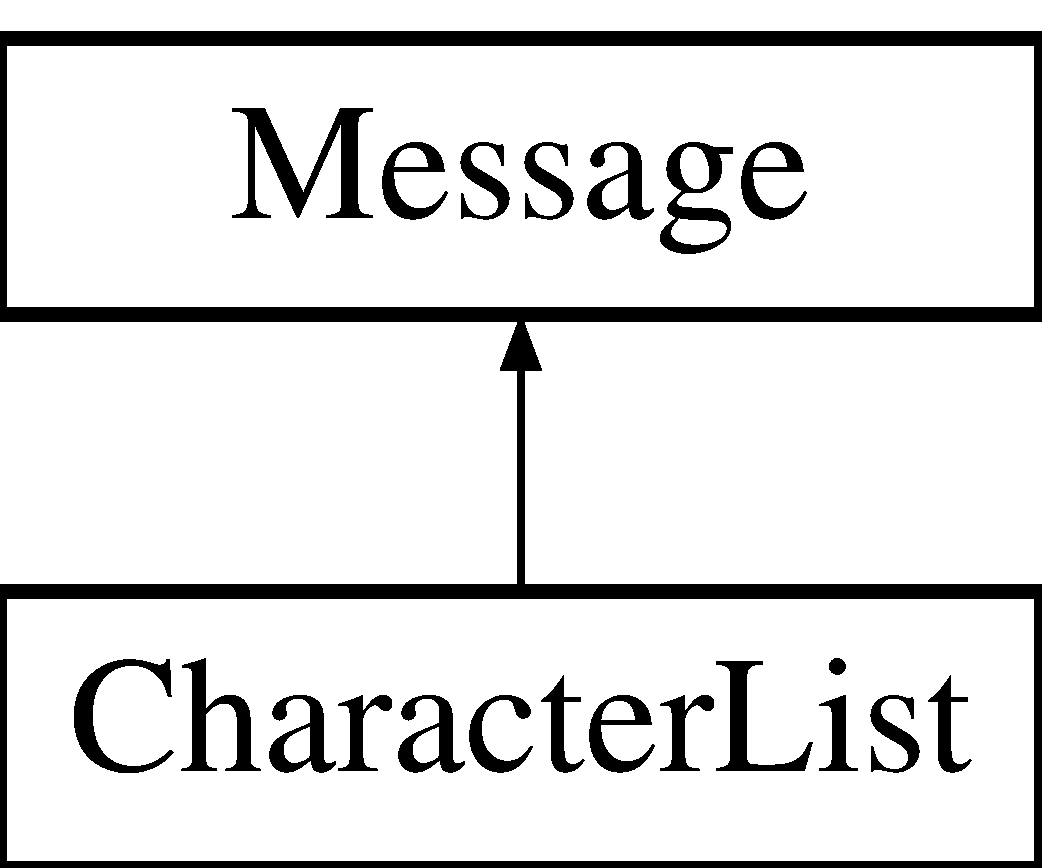
\includegraphics[height=2.000000cm]{classCharacterList}
\end{center}
\end{figure}
\subsection*{Public Member Functions}
\begin{DoxyCompactItemize}
\item 
{\bfseries Character\+List} (const \hyperlink{classCharacterList}{Character\+List} \&from)\hypertarget{classCharacterList_a1ed067e662cd53535231d97ebde90f3a}{}\label{classCharacterList_a1ed067e662cd53535231d97ebde90f3a}

\item 
\hyperlink{classCharacterList}{Character\+List} \& {\bfseries operator=} (const \hyperlink{classCharacterList}{Character\+List} \&from)\hypertarget{classCharacterList_a14a699dec984c891b62335324dce44c2}{}\label{classCharacterList_a14a699dec984c891b62335324dce44c2}

\item 
const \+::google\+::protobuf\+::\+Unknown\+Field\+Set \& {\bfseries unknown\+\_\+fields} () const \hypertarget{classCharacterList_a3c3975713049e07f49ecce655f2377b9}{}\label{classCharacterList_a3c3975713049e07f49ecce655f2377b9}

\item 
inline\+::google\+::protobuf\+::\+Unknown\+Field\+Set $\ast$ {\bfseries mutable\+\_\+unknown\+\_\+fields} ()\hypertarget{classCharacterList_ace97f06c2b340df27844b871f48f4f55}{}\label{classCharacterList_ace97f06c2b340df27844b871f48f4f55}

\item 
void {\bfseries Swap} (\hyperlink{classCharacterList}{Character\+List} $\ast$other)\hypertarget{classCharacterList_a09c3d2ac8f7c27358df80ddecdf05d8b}{}\label{classCharacterList_a09c3d2ac8f7c27358df80ddecdf05d8b}

\item 
\hyperlink{classCharacterList}{Character\+List} $\ast$ {\bfseries New} () const \hypertarget{classCharacterList_a02d238f38e24b848dfe937cbb0d338c9}{}\label{classCharacterList_a02d238f38e24b848dfe937cbb0d338c9}

\item 
void {\bfseries Copy\+From} (const \+::google\+::protobuf\+::\+Message \&from)\hypertarget{classCharacterList_a88a9e0cd7ac22adeb6ea757fe794c3e9}{}\label{classCharacterList_a88a9e0cd7ac22adeb6ea757fe794c3e9}

\item 
void {\bfseries Merge\+From} (const \+::google\+::protobuf\+::\+Message \&from)\hypertarget{classCharacterList_a665e578b3b4d25d8d066f0de52ed7f3c}{}\label{classCharacterList_a665e578b3b4d25d8d066f0de52ed7f3c}

\item 
void {\bfseries Copy\+From} (const \hyperlink{classCharacterList}{Character\+List} \&from)\hypertarget{classCharacterList_a562784317ca1d5a8a2f5d2e5c8dd4d91}{}\label{classCharacterList_a562784317ca1d5a8a2f5d2e5c8dd4d91}

\item 
void {\bfseries Merge\+From} (const \hyperlink{classCharacterList}{Character\+List} \&from)\hypertarget{classCharacterList_add64558c620d8c5e8e45dfbd90d4b286}{}\label{classCharacterList_add64558c620d8c5e8e45dfbd90d4b286}

\item 
void {\bfseries Clear} ()\hypertarget{classCharacterList_ad24a5a0cbd565eb9149c08f1decad097}{}\label{classCharacterList_ad24a5a0cbd565eb9149c08f1decad097}

\item 
bool {\bfseries Is\+Initialized} () const \hypertarget{classCharacterList_aed2311adb28f5438cb82a508bd42145a}{}\label{classCharacterList_aed2311adb28f5438cb82a508bd42145a}

\item 
int {\bfseries Byte\+Size} () const \hypertarget{classCharacterList_a4c6f0118b6b28a797f70d015c44d20b5}{}\label{classCharacterList_a4c6f0118b6b28a797f70d015c44d20b5}

\item 
bool {\bfseries Merge\+Partial\+From\+Coded\+Stream} (\+::google\+::protobuf\+::io\+::\+Coded\+Input\+Stream $\ast$input)\hypertarget{classCharacterList_aeb1ceec9c884d8639ea71fe30021bbee}{}\label{classCharacterList_aeb1ceec9c884d8639ea71fe30021bbee}

\item 
void {\bfseries Serialize\+With\+Cached\+Sizes} (\+::google\+::protobuf\+::io\+::\+Coded\+Output\+Stream $\ast$output) const \hypertarget{classCharacterList_a8ae35703c54b7c41078c3a382856226c}{}\label{classCharacterList_a8ae35703c54b7c41078c3a382856226c}

\item 
\+::google\+::protobuf\+::uint8 $\ast$ {\bfseries Serialize\+With\+Cached\+Sizes\+To\+Array} (\+::google\+::protobuf\+::uint8 $\ast$output) const \hypertarget{classCharacterList_a571a94b4fad69030b34364204ba095f6}{}\label{classCharacterList_a571a94b4fad69030b34364204ba095f6}

\item 
int {\bfseries Get\+Cached\+Size} () const \hypertarget{classCharacterList_afccf044b279943d127b9f3b3dda13836}{}\label{classCharacterList_afccf044b279943d127b9f3b3dda13836}

\item 
\+::google\+::protobuf\+::\+Metadata {\bfseries Get\+Metadata} () const \hypertarget{classCharacterList_adb5941fe37a628f8add547299178c3b6}{}\label{classCharacterList_adb5941fe37a628f8add547299178c3b6}

\item 
int {\bfseries character\+\_\+size} () const \hypertarget{classCharacterList_ac81e72b6db9cb80d4535f509d7f1f433}{}\label{classCharacterList_ac81e72b6db9cb80d4535f509d7f1f433}

\item 
void {\bfseries clear\+\_\+character} ()\hypertarget{classCharacterList_a174ebd6f142f1291b08f3198c02e2c26}{}\label{classCharacterList_a174ebd6f142f1291b08f3198c02e2c26}

\item 
const \+::\hyperlink{classCharacter}{Character} \& {\bfseries character} (int index) const \hypertarget{classCharacterList_a5594fe03d683c7b1d711c96c6039b9c8}{}\label{classCharacterList_a5594fe03d683c7b1d711c96c6039b9c8}

\item 
inline\+::\+Character $\ast$ {\bfseries mutable\+\_\+character} (int index)\hypertarget{classCharacterList_af4916b9b95cfe6243a465cd4f9a56cdf}{}\label{classCharacterList_af4916b9b95cfe6243a465cd4f9a56cdf}

\item 
inline\+::\+Character $\ast$ {\bfseries add\+\_\+character} ()\hypertarget{classCharacterList_aad299d4b8b21eb2349974bd9cd3187d7}{}\label{classCharacterList_aad299d4b8b21eb2349974bd9cd3187d7}

\item 
const \+::google\+::protobuf\+::\+Repeated\+Ptr\+Field$<$ \+::\hyperlink{classCharacter}{Character} $>$ \& {\bfseries character} () const \hypertarget{classCharacterList_a40c5d419b9d4a7ae03aaf699c3df7feb}{}\label{classCharacterList_a40c5d419b9d4a7ae03aaf699c3df7feb}

\item 
inline\+::google\+::protobuf\+::\+Repeated\+Ptr\+Field$<$ \+::\hyperlink{classCharacter}{Character} $>$ $\ast$ {\bfseries mutable\+\_\+character} ()\hypertarget{classCharacterList_a7a1ab42b9b5441fdeb8d8f3a95c4238c}{}\label{classCharacterList_a7a1ab42b9b5441fdeb8d8f3a95c4238c}

\end{DoxyCompactItemize}
\subsection*{Static Public Member Functions}
\begin{DoxyCompactItemize}
\item 
static const \+::google\+::protobuf\+::\+Descriptor $\ast$ {\bfseries descriptor} ()\hypertarget{classCharacterList_aace6de641ed334c6d6a4cbbe7714ca8b}{}\label{classCharacterList_aace6de641ed334c6d6a4cbbe7714ca8b}

\item 
static const \hyperlink{classCharacterList}{Character\+List} \& {\bfseries default\+\_\+instance} ()\hypertarget{classCharacterList_aa180968dade6512bfa0e9c21b57b0b84}{}\label{classCharacterList_aa180968dade6512bfa0e9c21b57b0b84}

\end{DoxyCompactItemize}
\subsection*{Static Public Attributes}
\begin{DoxyCompactItemize}
\item 
static const int {\bfseries k\+Character\+Field\+Number} = 5\hypertarget{classCharacterList_a4290f8fc798d31c54076ae65c2401ca3}{}\label{classCharacterList_a4290f8fc798d31c54076ae65c2401ca3}

\end{DoxyCompactItemize}
\subsection*{Friends}
\begin{DoxyCompactItemize}
\item 
void {\bfseries protobuf\+\_\+\+Add\+Desc\+\_\+\+Character\+Protobuf\+\_\+2eproto} ()\hypertarget{classCharacterList_aa491aa56977170cd80caf7b8176ae84c}{}\label{classCharacterList_aa491aa56977170cd80caf7b8176ae84c}

\item 
void {\bfseries protobuf\+\_\+\+Assign\+Desc\+\_\+\+Character\+Protobuf\+\_\+2eproto} ()\hypertarget{classCharacterList_a510135aa7690c32c0b8f2f1b539199aa}{}\label{classCharacterList_a510135aa7690c32c0b8f2f1b539199aa}

\item 
void {\bfseries protobuf\+\_\+\+Shutdown\+File\+\_\+\+Character\+Protobuf\+\_\+2eproto} ()\hypertarget{classCharacterList_aa03453ef0dc13477cc670111c24af42a}{}\label{classCharacterList_aa03453ef0dc13477cc670111c24af42a}

\end{DoxyCompactItemize}


The documentation for this class was generated from the following files\+:\begin{DoxyCompactItemize}
\item 
Character\+Protobuf.\+pb.\+h\item 
Character\+Protobuf.\+pb.\+cc\end{DoxyCompactItemize}

\hypertarget{classCharacterPrototype}{}\section{Character\+Prototype Class Reference}
\label{classCharacterPrototype}\index{Character\+Prototype@{Character\+Prototype}}


{\ttfamily \#include $<$Character\+Prototype.\+h$>$}

Inheritance diagram for Character\+Prototype\+:\begin{figure}[H]
\begin{center}
\leavevmode
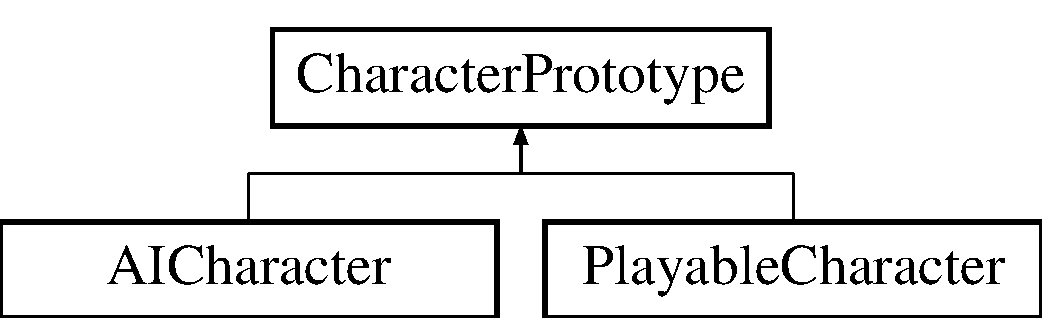
\includegraphics[height=2.000000cm]{classCharacterPrototype}
\end{center}
\end{figure}
\subsection*{Public Member Functions}
\begin{DoxyCompactItemize}
\item 
\hyperlink{classCharacterPrototype_a6485d2e9c20779dc8f56943e63929e62}{Character\+Prototype} (std\+::string name, std\+::string type)
\item 
\hyperlink{classCharacterPrototype_abe3e17663cb992859d4fc3f3271e70e3}{Character\+Prototype} (const \hyperlink{classCharacterPrototype}{Character\+Prototype} \&orig)
\item 
virtual \hyperlink{classCharacterPrototype}{Character\+Prototype} $\ast$ \hyperlink{classCharacterPrototype_a7c3db310af19ff8c80eb3a7f20bd9986}{clone} ()=0
\item 
virtual void \hyperlink{classCharacterPrototype_aa656ad04dd911f24f2885dec50027bd8}{set\+Name} (std\+::string name)
\item 
virtual std\+::string \hyperlink{classCharacterPrototype_a97dd213c4515c631eac8957fec5d83fe}{get\+Name} ()
\item 
virtual std\+::string \hyperlink{classCharacterPrototype_abec1a7dacbee3aac9e67c75861b77ff1}{get\+Type} ()
\item 
virtual \hyperlink{classCharacterPrototype_a07cc2f45577611f264a954b1ff45777a}{$\sim$\+Character\+Prototype} ()
\end{DoxyCompactItemize}
\subsection*{Protected Attributes}
\begin{DoxyCompactItemize}
\item 
std\+::string {\bfseries name}\hypertarget{classCharacterPrototype_a38e7079fcedaaaa30e9af6b8f55e9790}{}\label{classCharacterPrototype_a38e7079fcedaaaa30e9af6b8f55e9790}

\item 
std\+::string {\bfseries type}\hypertarget{classCharacterPrototype_ac827564d5db88558075e89052a4d4eda}{}\label{classCharacterPrototype_ac827564d5db88558075e89052a4d4eda}

\end{DoxyCompactItemize}


\subsection{Detailed Description}
The base class \hyperlink{classCharacter}{Character} Prototype 

\subsection{Constructor \& Destructor Documentation}
\index{Character\+Prototype@{Character\+Prototype}!Character\+Prototype@{Character\+Prototype}}
\index{Character\+Prototype@{Character\+Prototype}!Character\+Prototype@{Character\+Prototype}}
\subsubsection[{Character\+Prototype(std\+::string name, std\+::string type)}]{\setlength{\rightskip}{0pt plus 5cm}Character\+Prototype\+::\+Character\+Prototype (
\begin{DoxyParamCaption}
\item[{std\+::string}]{name, }
\item[{std\+::string}]{type}
\end{DoxyParamCaption}
)}\hypertarget{classCharacterPrototype_a6485d2e9c20779dc8f56943e63929e62}{}\label{classCharacterPrototype_a6485d2e9c20779dc8f56943e63929e62}
Create a new character prototype 
\begin{DoxyParams}{Parameters}
{\em name} & the name of the character \\
\hline
{\em type} & the type of the character \\
\hline
\end{DoxyParams}
\index{Character\+Prototype@{Character\+Prototype}!Character\+Prototype@{Character\+Prototype}}
\index{Character\+Prototype@{Character\+Prototype}!Character\+Prototype@{Character\+Prototype}}
\subsubsection[{Character\+Prototype(const Character\+Prototype \&orig)}]{\setlength{\rightskip}{0pt plus 5cm}Character\+Prototype\+::\+Character\+Prototype (
\begin{DoxyParamCaption}
\item[{const {\bf Character\+Prototype} \&}]{orig}
\end{DoxyParamCaption}
)}\hypertarget{classCharacterPrototype_abe3e17663cb992859d4fc3f3271e70e3}{}\label{classCharacterPrototype_abe3e17663cb992859d4fc3f3271e70e3}
Copies a new character prototype 
\begin{DoxyParams}{Parameters}
{\em orig} & a reference to the character to copy \\
\hline
\end{DoxyParams}
\index{Character\+Prototype@{Character\+Prototype}!````~Character\+Prototype@{$\sim$\+Character\+Prototype}}
\index{````~Character\+Prototype@{$\sim$\+Character\+Prototype}!Character\+Prototype@{Character\+Prototype}}
\subsubsection[{$\sim$\+Character\+Prototype()}]{\setlength{\rightskip}{0pt plus 5cm}Character\+Prototype\+::$\sim$\+Character\+Prototype (
\begin{DoxyParamCaption}
{}
\end{DoxyParamCaption}
)\hspace{0.3cm}{\ttfamily [virtual]}}\hypertarget{classCharacterPrototype_a07cc2f45577611f264a954b1ff45777a}{}\label{classCharacterPrototype_a07cc2f45577611f264a954b1ff45777a}
Deletes the character 

\subsection{Member Function Documentation}
\index{Character\+Prototype@{Character\+Prototype}!clone@{clone}}
\index{clone@{clone}!Character\+Prototype@{Character\+Prototype}}
\subsubsection[{clone()=0}]{\setlength{\rightskip}{0pt plus 5cm}virtual {\bf Character\+Prototype}$\ast$ Character\+Prototype\+::clone (
\begin{DoxyParamCaption}
{}
\end{DoxyParamCaption}
)\hspace{0.3cm}{\ttfamily [pure virtual]}}\hypertarget{classCharacterPrototype_a7c3db310af19ff8c80eb3a7f20bd9986}{}\label{classCharacterPrototype_a7c3db310af19ff8c80eb3a7f20bd9986}
Clones a new character prototype, must be implemented by derived classes \begin{DoxyReturn}{Returns}
A clone of the character 
\end{DoxyReturn}


Implemented in \hyperlink{classAICharacter_a99b6f645c4e1f24d9701bac8f0dee596}{A\+I\+Character}, and \hyperlink{classPlayableCharacter_aadde0d9220aa0dd78b51bbbe87ecd628}{Playable\+Character}.

\index{Character\+Prototype@{Character\+Prototype}!get\+Name@{get\+Name}}
\index{get\+Name@{get\+Name}!Character\+Prototype@{Character\+Prototype}}
\subsubsection[{get\+Name()}]{\setlength{\rightskip}{0pt plus 5cm}std\+::string Character\+Prototype\+::get\+Name (
\begin{DoxyParamCaption}
{}
\end{DoxyParamCaption}
)\hspace{0.3cm}{\ttfamily [virtual]}}\hypertarget{classCharacterPrototype_a97dd213c4515c631eac8957fec5d83fe}{}\label{classCharacterPrototype_a97dd213c4515c631eac8957fec5d83fe}
Get character\textquotesingle{}s name \begin{DoxyReturn}{Returns}
the character\textquotesingle{}s name 
\end{DoxyReturn}
\index{Character\+Prototype@{Character\+Prototype}!get\+Type@{get\+Type}}
\index{get\+Type@{get\+Type}!Character\+Prototype@{Character\+Prototype}}
\subsubsection[{get\+Type()}]{\setlength{\rightskip}{0pt plus 5cm}std\+::string Character\+Prototype\+::get\+Type (
\begin{DoxyParamCaption}
{}
\end{DoxyParamCaption}
)\hspace{0.3cm}{\ttfamily [virtual]}}\hypertarget{classCharacterPrototype_abec1a7dacbee3aac9e67c75861b77ff1}{}\label{classCharacterPrototype_abec1a7dacbee3aac9e67c75861b77ff1}
Get character\textquotesingle{}s type \begin{DoxyReturn}{Returns}
the character\textquotesingle{}s type 
\end{DoxyReturn}
\index{Character\+Prototype@{Character\+Prototype}!set\+Name@{set\+Name}}
\index{set\+Name@{set\+Name}!Character\+Prototype@{Character\+Prototype}}
\subsubsection[{set\+Name(std\+::string name)}]{\setlength{\rightskip}{0pt plus 5cm}void Character\+Prototype\+::set\+Name (
\begin{DoxyParamCaption}
\item[{std\+::string}]{name}
\end{DoxyParamCaption}
)\hspace{0.3cm}{\ttfamily [virtual]}}\hypertarget{classCharacterPrototype_aa656ad04dd911f24f2885dec50027bd8}{}\label{classCharacterPrototype_aa656ad04dd911f24f2885dec50027bd8}
Set character\textquotesingle{}s name 
\begin{DoxyParams}{Parameters}
{\em name} & the new name \\
\hline
\end{DoxyParams}


The documentation for this class was generated from the following files\+:\begin{DoxyCompactItemize}
\item 
Character\+Prototype.\+h\item 
Character\+Prototype.\+cpp\end{DoxyCompactItemize}

\hypertarget{classCharacterPrototypeFactory}{}\section{Character\+Prototype\+Factory Class Reference}
\label{classCharacterPrototypeFactory}\index{Character\+Prototype\+Factory@{Character\+Prototype\+Factory}}


{\ttfamily \#include $<$Character\+Prototype\+Factory.\+h$>$}

\subsection*{Public Member Functions}
\begin{DoxyCompactItemize}
\item 
\hyperlink{classCharacterPrototypeFactory_a0980d1087a9a5456cb151fcf5b4b0a6d}{Character\+Prototype\+Factory} ()
\item 
{\bfseries Character\+Prototype\+Factory} (const \hyperlink{classCharacterPrototypeFactory}{Character\+Prototype\+Factory} \&orig)\hypertarget{classCharacterPrototypeFactory_a488cb5f74bda3a6c8594745a84c79a9f}{}\label{classCharacterPrototypeFactory_a488cb5f74bda3a6c8594745a84c79a9f}

\item 
virtual \hyperlink{classCharacterPrototype}{Character\+Prototype} $\ast$ \hyperlink{classCharacterPrototypeFactory_a4d2046b26fa5c620ef35719c3893c03c}{get\+Playable} ()
\item 
virtual \hyperlink{classCharacterPrototype}{Character\+Prototype} $\ast$ \hyperlink{classCharacterPrototypeFactory_a1101cdf1640bed732c339b9994c6bb1e}{get\+AI} ()
\item 
virtual \hyperlink{classCharacterPrototypeFactory_aafffdccd0b32a145f3fb8d38002cf761}{$\sim$\+Character\+Prototype\+Factory} ()
\end{DoxyCompactItemize}


\subsection{Detailed Description}
A Prototype Factory for \hyperlink{classCharacter}{Character} Prototypes 

\subsection{Constructor \& Destructor Documentation}
\index{Character\+Prototype\+Factory@{Character\+Prototype\+Factory}!Character\+Prototype\+Factory@{Character\+Prototype\+Factory}}
\index{Character\+Prototype\+Factory@{Character\+Prototype\+Factory}!Character\+Prototype\+Factory@{Character\+Prototype\+Factory}}
\subsubsection[{Character\+Prototype\+Factory()}]{\setlength{\rightskip}{0pt plus 5cm}Character\+Prototype\+Factory\+::\+Character\+Prototype\+Factory (
\begin{DoxyParamCaption}
{}
\end{DoxyParamCaption}
)}\hypertarget{classCharacterPrototypeFactory_a0980d1087a9a5456cb151fcf5b4b0a6d}{}\label{classCharacterPrototypeFactory_a0980d1087a9a5456cb151fcf5b4b0a6d}
Creates a \hyperlink{classCharacter}{Character} Prototype Factory \index{Character\+Prototype\+Factory@{Character\+Prototype\+Factory}!````~Character\+Prototype\+Factory@{$\sim$\+Character\+Prototype\+Factory}}
\index{````~Character\+Prototype\+Factory@{$\sim$\+Character\+Prototype\+Factory}!Character\+Prototype\+Factory@{Character\+Prototype\+Factory}}
\subsubsection[{$\sim$\+Character\+Prototype\+Factory()}]{\setlength{\rightskip}{0pt plus 5cm}Character\+Prototype\+Factory\+::$\sim$\+Character\+Prototype\+Factory (
\begin{DoxyParamCaption}
{}
\end{DoxyParamCaption}
)\hspace{0.3cm}{\ttfamily [virtual]}}\hypertarget{classCharacterPrototypeFactory_aafffdccd0b32a145f3fb8d38002cf761}{}\label{classCharacterPrototypeFactory_aafffdccd0b32a145f3fb8d38002cf761}
Destroys the \hyperlink{classCharacter}{Character} Prototype 

\subsection{Member Function Documentation}
\index{Character\+Prototype\+Factory@{Character\+Prototype\+Factory}!get\+AI@{get\+AI}}
\index{get\+AI@{get\+AI}!Character\+Prototype\+Factory@{Character\+Prototype\+Factory}}
\subsubsection[{get\+A\+I()}]{\setlength{\rightskip}{0pt plus 5cm}{\bf Character\+Prototype} $\ast$ Character\+Prototype\+Factory\+::get\+AI (
\begin{DoxyParamCaption}
{}
\end{DoxyParamCaption}
)\hspace{0.3cm}{\ttfamily [virtual]}}\hypertarget{classCharacterPrototypeFactory_a1101cdf1640bed732c339b9994c6bb1e}{}\label{classCharacterPrototypeFactory_a1101cdf1640bed732c339b9994c6bb1e}
Creates a clone of a default AI character \begin{DoxyReturn}{Returns}
a default AI character clone 
\end{DoxyReturn}
\index{Character\+Prototype\+Factory@{Character\+Prototype\+Factory}!get\+Playable@{get\+Playable}}
\index{get\+Playable@{get\+Playable}!Character\+Prototype\+Factory@{Character\+Prototype\+Factory}}
\subsubsection[{get\+Playable()}]{\setlength{\rightskip}{0pt plus 5cm}{\bf Character\+Prototype} $\ast$ Character\+Prototype\+Factory\+::get\+Playable (
\begin{DoxyParamCaption}
{}
\end{DoxyParamCaption}
)\hspace{0.3cm}{\ttfamily [virtual]}}\hypertarget{classCharacterPrototypeFactory_a4d2046b26fa5c620ef35719c3893c03c}{}\label{classCharacterPrototypeFactory_a4d2046b26fa5c620ef35719c3893c03c}
Creates a clone of a default playable character \begin{DoxyReturn}{Returns}
a default playable character clone 
\end{DoxyReturn}


The documentation for this class was generated from the following files\+:\begin{DoxyCompactItemize}
\item 
Character\+Prototype\+Factory.\+h\item 
Character\+Prototype\+Factory.\+cpp\end{DoxyCompactItemize}

\hypertarget{classPlayableCharacter}{}\section{Playable\+Character Class Reference}
\label{classPlayableCharacter}\index{Playable\+Character@{Playable\+Character}}


{\ttfamily \#include $<$Playable\+Character.\+h$>$}

Inheritance diagram for Playable\+Character\+:\begin{figure}[H]
\begin{center}
\leavevmode
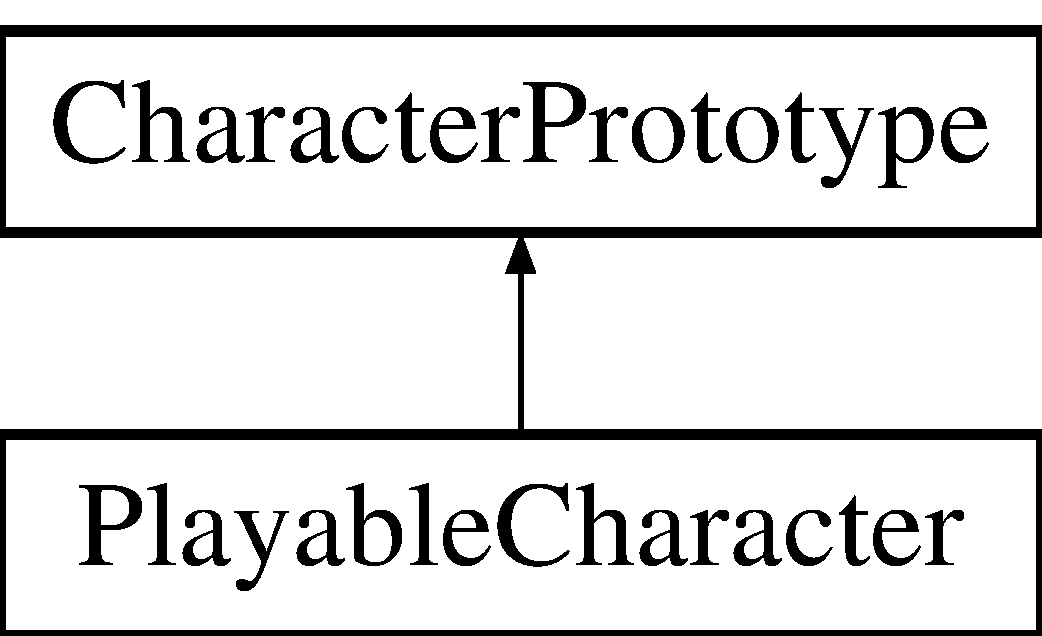
\includegraphics[height=2.000000cm]{classPlayableCharacter}
\end{center}
\end{figure}
\subsection*{Public Member Functions}
\begin{DoxyCompactItemize}
\item 
\hyperlink{classPlayableCharacter_a2c03ac78c7f71376ba874026693122c9}{Playable\+Character} (std\+::string name)
\item 
\hyperlink{classPlayableCharacter_afea57d110e99ca826e37e077f2787fa2}{Playable\+Character} (const \hyperlink{classPlayableCharacter}{Playable\+Character} \&orig)
\item 
virtual \hyperlink{classCharacterPrototype}{Character\+Prototype} $\ast$ \hyperlink{classPlayableCharacter_aadde0d9220aa0dd78b51bbbe87ecd628}{clone} ()
\item 
virtual \hyperlink{classPlayableCharacter_aa738dea6ac366827ca4a7f6ad406bba2}{$\sim$\+Playable\+Character} ()
\end{DoxyCompactItemize}
\subsection*{Additional Inherited Members}


\subsection{Detailed Description}
Playable \hyperlink{classCharacter}{Character}, a derived class from \hyperlink{classCharacter}{Character} Prototype 

\subsection{Constructor \& Destructor Documentation}
\index{Playable\+Character@{Playable\+Character}!Playable\+Character@{Playable\+Character}}
\index{Playable\+Character@{Playable\+Character}!Playable\+Character@{Playable\+Character}}
\subsubsection[{Playable\+Character(std\+::string name)}]{\setlength{\rightskip}{0pt plus 5cm}Playable\+Character\+::\+Playable\+Character (
\begin{DoxyParamCaption}
\item[{std\+::string}]{name}
\end{DoxyParamCaption}
)}\hypertarget{classPlayableCharacter_a2c03ac78c7f71376ba874026693122c9}{}\label{classPlayableCharacter_a2c03ac78c7f71376ba874026693122c9}
Creates a new playable character 
\begin{DoxyParams}{Parameters}
{\em name} & the name for the player \\
\hline
\end{DoxyParams}
\index{Playable\+Character@{Playable\+Character}!Playable\+Character@{Playable\+Character}}
\index{Playable\+Character@{Playable\+Character}!Playable\+Character@{Playable\+Character}}
\subsubsection[{Playable\+Character(const Playable\+Character \&orig)}]{\setlength{\rightskip}{0pt plus 5cm}Playable\+Character\+::\+Playable\+Character (
\begin{DoxyParamCaption}
\item[{const {\bf Playable\+Character} \&}]{orig}
\end{DoxyParamCaption}
)}\hypertarget{classPlayableCharacter_afea57d110e99ca826e37e077f2787fa2}{}\label{classPlayableCharacter_afea57d110e99ca826e37e077f2787fa2}
Copies a playable character 
\begin{DoxyParams}{Parameters}
{\em orig} & the playable character to copy \\
\hline
\end{DoxyParams}
\index{Playable\+Character@{Playable\+Character}!````~Playable\+Character@{$\sim$\+Playable\+Character}}
\index{````~Playable\+Character@{$\sim$\+Playable\+Character}!Playable\+Character@{Playable\+Character}}
\subsubsection[{$\sim$\+Playable\+Character()}]{\setlength{\rightskip}{0pt plus 5cm}Playable\+Character\+::$\sim$\+Playable\+Character (
\begin{DoxyParamCaption}
{}
\end{DoxyParamCaption}
)\hspace{0.3cm}{\ttfamily [virtual]}}\hypertarget{classPlayableCharacter_aa738dea6ac366827ca4a7f6ad406bba2}{}\label{classPlayableCharacter_aa738dea6ac366827ca4a7f6ad406bba2}
Destroys the character 

\subsection{Member Function Documentation}
\index{Playable\+Character@{Playable\+Character}!clone@{clone}}
\index{clone@{clone}!Playable\+Character@{Playable\+Character}}
\subsubsection[{clone()}]{\setlength{\rightskip}{0pt plus 5cm}{\bf Character\+Prototype} $\ast$ Playable\+Character\+::clone (
\begin{DoxyParamCaption}
{}
\end{DoxyParamCaption}
)\hspace{0.3cm}{\ttfamily [virtual]}}\hypertarget{classPlayableCharacter_aadde0d9220aa0dd78b51bbbe87ecd628}{}\label{classPlayableCharacter_aadde0d9220aa0dd78b51bbbe87ecd628}
Clones the playable character \begin{DoxyReturn}{Returns}
a clone of the character 
\end{DoxyReturn}


Implements \hyperlink{classCharacterPrototype_a7c3db310af19ff8c80eb3a7f20bd9986}{Character\+Prototype}.



The documentation for this class was generated from the following files\+:\begin{DoxyCompactItemize}
\item 
Playable\+Character.\+h\item 
Playable\+Character.\+cpp\end{DoxyCompactItemize}

\hypertarget{structStaticDescriptorInitializer__CharacterProtobuf__2eproto}{}\section{Static\+Descriptor\+Initializer\+\_\+\+Character\+Protobuf\+\_\+2eproto Struct Reference}
\label{structStaticDescriptorInitializer__CharacterProtobuf__2eproto}\index{Static\+Descriptor\+Initializer\+\_\+\+Character\+Protobuf\+\_\+2eproto@{Static\+Descriptor\+Initializer\+\_\+\+Character\+Protobuf\+\_\+2eproto}}


The documentation for this struct was generated from the following file\+:\begin{DoxyCompactItemize}
\item 
Character\+Protobuf.\+pb.\+cc\end{DoxyCompactItemize}

%--- End generated contents ---

% Index
\backmatter
\newpage
\phantomsection
\clearemptydoublepage
\addcontentsline{toc}{chapter}{Index}
\printindex

\end{document}
